% This is samplepaper.tex, a sample chapter demonstrating the
% LLNCS macro package for Springer Computer Science proceedings;
% Version 2.21 of 2022/01/12
%
\documentclass[runningheads]{llncs}

% 数学相关
\usepackage{amsmath, amsfonts, bm, amssymb}

% 图形与表格
\usepackage{graphicx, svg}
\usepackage{array, booktabs, multirow}
\usepackage{stfloats}
\usepackage{subcaption}
\usepackage{multicol}

% 算法环境（推荐新写法）
\usepackage{algorithm}
\usepackage{algpseudocode} % 替换 algorithmic

% 字体与符号
\usepackage[T1]{fontenc}
\usepackage{textcomp, pifont}
\usepackage{enumitem}
% \usepackage{xeCJK}
\usepackage{CJKutf8}

% 引用与超链接
\usepackage{cite, url}

% 其他功能
\usepackage{pdfpages}
\usepackage{verbatim}
\usepackage{xcolor} % 保留一次
\usepackage{soul}

% ===========================
% 自定义命令与符号
% ===========================
% 圆形符号
\usepackage{tikz}
\newcommand*\emptycirc[1][1ex]{\tikz\draw (0,0) circle (#1);} 
\newcommand*\halfcirc[1][1ex]{%
    \begin{tikzpicture}
    \draw[fill] (0,0)-- (90:#1) arc (90:270:#1) -- cycle ;
    \draw (0,0) circle (#1);
    \end{tikzpicture}}
\newcommand*\fullcirc[1][1ex]{\tikz\fill (0,0) circle (#1);}

% 其他符号
\newcommand{\sharesig}{\mathsf{ShareSig}}
\newcommand{\ta}{\mathsf{TA}}
\newcommand{\txr}{\mathsf{TX}_r^I}
\newcommand{\blockr}{\mathsf{B}_r^I}
\newcommand{\blockrr}{\mathsf{B}_{r-1}^I}
\newcommand{\blockrrr}{\mathsf{B}_{r-2}^I}
\newcommand{\mprop}{m_\text{prop}}
\newcommand{\propose}{\mathtt{PROPOSE}}
\newcommand{\sigmaI}{{\sigma_I}}
\newcommand{\mpre}{m_\text{pre}}
\newcommand{\prepare}{\mathtt{PREPARE}}
\newcommand{\sigmai}{{\sigma_i}}
\newcommand{\recon}{\mathsf{Reconstruct}}
\newcommand{\Sigmapre}{\Sigma_\text{pre}}
\newcommand{\prepared}{\mathbf{prepared}}
\newcommand{\mcom}{m_\text{com}}
\newcommand{\commit}{\mathtt{COMMIT}}
\newcommand{\committed}{\mathbf{committed}}
\newcommand{\vote}{\mathtt{VOTE}}
\newcommand{\Sigmacom}{\Sigma_\text{com}}
\newcommand{\mvote}{m_\text{vote}}
\newcommand{\Sigmarr}{\Sigma_{r-1}}
\newcommand{\Sigmar}{\Sigma_{r}}
\newcommand{\inl}{{I\in[n_L]}}
\newcommand{\blockrnl}{\mathsf{B}_r^{n_L}}
\newcommand{\bft}{\mathsf{BFT}}
\newcommand{\bblockr}{\overline{\mathsf{B}}_r^I}
\newcommand{\DRG}{\mathsf{DRG}}
\newcommand{\setup}{\mathsf{Setup}}
\newcommand{\kzg}{\mathsf{KZG}}
\newcommand{\nizk}{\mathsf{NIZK}}
\newcommand{\nizkvf}{\mathsf{NIZK.Vf}}
\newcommand{\zksnark}{\mathsf{zkSNARK}}
\newcommand{\bg}{\mathbb{G}}
\newcommand{\ff}{\mathbb{F}}
\newcommand{\keygen}{\mathsf{KeyGen}}
\newcommand{\kzgcommit}{\mathsf{Commit}}
\newcommand{\decrypt}{\mathsf{Decrypt}}
\newcommand{\hash}{\mathsf{H}}
\newcommand{\vrf}{\mathsf{VRF}}
\newcommand{\ser}{\mathsf{Ser}}

% 颜色定义
\usepackage{xcolor}
\definecolor{mygray}{gray}{0.6}
\definecolor{yellow}{rgb}{0.9, 0.7, 0.0}
\definecolor{green}{rgb}{0.0, 0.5, 0.0}
\definecolor{purple}{rgb}{0.75, 0.0, 0.75}


%
\begin{document}
\begin{CJK*}{UTF8}{gbsn}

\title{AnoST: An Anonymous Optimistic Verification System Based on Off-Chain State Transition}


\author{Qiyuan Gao\inst{1} \and
Qianhong Wu\inst{1} \and
Junxiang Nong\inst{2} \and
Qi Liu\inst{1}
}

\authorrunning{Q. Gao et al.}

\institute{Beihang University, Beijing, China \and
Renmin University of China, Beijing, China\\
\email{gaoqy@buaa.edu.cn, qianhong.wu@buaa.edu.cn, liuqi2032472260@163.com, fpdqwq@yeah.net}
}

\maketitle              % typeset the header of the contribution
%


\begin{abstract}

Current blockchain optimistic verification schemes typically face critical challenges such as inadequate verifier workload verification, verifier identity exposure risks, and low transaction acceptance rates due to batch rollbacks, significantly impacting off-chain verification efficiency and security. To address these issues, we propose AnoST, an efficient transaction verification mechanism with enhanced verifier anonymity protection. First, we introduce an anonymous staking-based verifier election mechanism to preserve verifier privacy and mitigate identity exposure risks. Second, we propose a State Transition Commitment (STC) mechanism, enabling direct blockchain verification of verifier workloads, effectively resolving the Verifier's Dilemma (Luu et al., CCS 2015). Furthermore, we develop a partial rollback mechanism leveraging State Transition Trees (STT), significantly improving transaction acceptance rates and system efficiency. Experimental results demonstrate that AnoST achieves notable advantages in security, anonymity protection, and transaction approval rates, highlighting its promising practicality and scalability.

\keywords{Blockchain Rollup, Optimistic Verification, Verifier's Dilemma}

\end{abstract}

\section{Introduction}

In recent years, with the rapid development of distributed computing technologies, third-party applications have increasingly required reliable and efficient verification of computation results~\cite{du2001privacy, kissner2005privacy, backes2016reliable, mcallister2012regulation, setty2012taking, yu2017survey}.  Blockchain~\cite{blk1,blk2,blk3}, characterized by decentralization, transparency, and tamper-resistance, has emerged as a mainstream solution for computational verification, finding widespread application in edge computing~\cite{edge1,edge2,edge3}, federated learning~\cite{fed1,fed2,fed3}, decentralized finance (DeFi)~\cite{defi1}, and other domains.

However, the traditional verification model of blockchain, constrained by factors such as independent node computation, limited block capacity~\cite{size1,size2}, and consensus mechanisms~\cite{con1,con2,con3,con4}, exhibits significant performance bottlenecks, failing to meet the growing demand for efficient verification. To mitigate these issues, verification schemes represented by Optimistic Rollup~\cite{op1,op2} have been proposed. Optimistic Rollup transfers complex computational tasks off-chain, submitting only the final state commitment on-chain and employing fraud-proof mechanisms when disputes arise, greatly enhancing on-chain verification efficiency and transaction throughput.

Despite these advantages, current Optimistic Rollup implementations still face several critical challenges in practical deployments. First, insufficient economic incentives for verifiers conducting off-chain validations often lead to the \emph{Verifier's Dilemma}~\cite{dilemma,dilemma1}, where rational verifiers tend to avoid actively performing validations, thereby compromising system security. Second, the absence of anonymity protection mechanisms for verifiers makes them vulnerable targets for malicious attacks, significantly increasing security risks. Furthermore, the prevailing batch rollback mechanisms reject entire transaction batches due to individual faulty transactions, severely impacting the approval rate of valid transactions.

\subsection{Problem Statement}

In this section, we will analyze and distill the issues identified above, in order to clearly define the design objectives for our solution.

\textbf{Verifier Identity Exposure and Security Risks.}  
Optimistic Rollup relies on verifiers to monitor off-chain transactions and submit fraud proofs to prevent fraudulent states from being committed on-chain. However, blockchain Publicity leads to exposure of verifier identities~\cite{id1,id2}, making them susceptible to bribery, targeted attacks, or even internal collusion. Such risks severely undermine the security and reliability of the verification process, ultimately threatening the overall system stability.

\textbf{Verifier's Dilemma.}  
The Verifier's Dilemma arises when rational verifiers choose not to actively verify transactions due to cost considerations, especially when the majority of transactions are expected to be correct. Verifiers tend to rely on others to perform verification tasks, creating collective inaction. If all verifiers adopt this strategy, the system may lack adequate oversight, allowing error transactions to successfully enter the blockchain and significantly diminishing the system's security and integrity.

\textbf{Excessive Verification Period and Batch Rollback Issues.}  
Current Optimistic Rollup schemes typically enforce prolonged verification dispute periods, involving multiple interactive rounds on-chain to identify disputed transactions. This results in significant delays in final transaction confirmations, substantially affecting system throughput and verification efficiency. Additionally, if a transaction batch contains erroneous transactions, the entire batch is rejected, dramatically reducing the throughput efficiency of valid transactions and negatively impacting overall system performance.

Therefore, designing an efficient off-chain transaction verification mechanism that ensures verifier anonymity and effectively incentivizes active participation from verifiers has become a critical and urgent issue for blockchain-based Optimistic Rollup solutions.

\subsection{Our Contributions}
In summary, designing an efficient verification mechanism that ensures verifier anonymity while incentivizing proactive verifier participation has emerged as a critical challenge in off-chain scaling solutions. To address this, we propose the AnoST with the following major contributions:

\begin{enumerate}
    \item We introduce an anonymous staking-based verifier election mechanism, which ensures verifier identity anonymity throughout the verification process, fundamentally mitigating bribery, collusion, and targeted attack risks associated with verifier identity exposure.

    \item We propose an on-chain verification mechanism leveraging the State Transition Commitment (STC). Through this mechanism, the blockchain can directly verify the actual workload performed by off-chain verifiers by comparing state commitment hashes, effectively resolving the verifier's dilemma.

    \item Building upon the STC mechanism, we further design a refined partial confirmation and rollback scheme using the State Transition Tree (STT). With this scheme, when erroneous transactions are detected in a batch, the system precisely rolls back only the incorrect states and their dependent transactions, thus significantly enhancing the overall transaction throughput and verification efficiency.

    \item We conduct comprehensive experimental analyses on AnoST. The results demonstrate that our mechanism achieves acceptable on-chain computational and storage overhead, while providing highly efficient transaction verification performance, confirming its practical effectiveness.
\end{enumerate}



\section{Preliminaries}

\subsection{Optimistic Rollup}

Optimistic Rollup~\cite{op-url} is a widely adopted blockchain scaling solution that improves throughput by executing transactions off-chain and submitting only state commitments on-chain. It operates under the assumption that transactions are valid unless challenged, triggering on-chain fraud proofs only when disputes arise. This design significantly reduces on-chain computation while preserving correctness.

Table~\ref{tab:comparison} compares several representative protocols. Most systems expose verifier identities and lack mechanisms to enforce honest verification, leading to the Verifier’s Dilemma. Arbitrum introduces interactive dispute resolution with logarithmic complexity, while others, including AnoST, support one-shot challenges. Only AnoST ensures verifier anonymity, proves verification effort via STC, and supports precise transaction-level rollback for efficient error localization.

\begin{table*}[t]
\centering
\caption{Comparison of Optimistic Verification Protocols}
\label{tab:comparison}
\renewcommand{\arraystretch}{1.3}
\begin{tabular}{p{10em}  p{6em}  p{7.5em}  p{6.5em}  p{6em}}
\toprule
\textbf{Feature} & \textbf{Optimism}~\cite{op-url} & \textbf{Arbitrum}~\cite{arbitrum} & \textbf{Cartesi}~\cite{cartesi} & \textbf{AnoST} \\
\midrule
\textbf{Verifier Identity} & Public Addr & Public Addr & Public Addr & Anony ID \\

\textbf{Verifier's Dilemma} & \ding{55} & \ding{51}  & \ding{55} & \ding{51} \\

\textbf{Challenge Round} & O(1) & O(log n)  & O(1)  & O(1) \\

\textbf{Proof Method} & Tx Re-exe & VM-step & Vm-Segment & Tx Re-exe \\

\textbf{Rollback} & \ding{55} & \ding{55} & \ding{55} & \ding{51}  \\
\bottomrule
\end{tabular}
\end{table*}




\subsection{Aztec Private Transfers}
Aztec~\cite{aztec} enables confidential asset transfers on Ethereum by representing each asset as a note:$N = \textsf{Commit}(v, \rho, pk)$, where \( v \) is the value, \( \rho \) is randomness, and \( pk \) is the recipient’s public key. A private transfer consumes input notes \( \{N_i\} \) and creates output notes \( \{N_j'\} \), preserving value: $\sum_i v_i = \sum_j v_j'$. A zero-knowledge proof \( \pi \) is generated to prove correctness and ownership without revealing \( v \), \( \rho \), or \( pk \). This construction guarantees value privacy, sender/receiver anonymity, and public verifiability.


\section{Definitions and System Model}

We consider a set of verifiers in the system, denoted as $\mathcal{V} = \{V_1, V_2, \dots, V_m\}$. Each verifier $V_i \in \mathcal{V}$ is assumed to be rational, meaning they always make decisions aimed at maximizing their own economic benefit. A verification task $\mathcal{T}$ (hereinafter referred to as transaction set) is defined as a set of transactions to be verified, i.e., $\mathcal{T} = \{\tau_1, \tau_2, \dots, \tau_n\}$, where each transaction $\tau_i$ triggers an update to the system state upon execution. Moreover, we assume that economic incentives provided by the system fully cover the costs incurred by honest executors and verifiers.

To clearly define the analytical scope and preconditions of this paper, we introduce the following two fundamental assumptions:

\textbf{Assumption 1 (Blockchain Trust Assumption):} 
We assume the consensus mechanism of the underlying blockchain is secure and trustworthy, meaning attackers cannot modify or revoke states that have been finalized by the blockchain's consensus protocol. Consequently, any transaction result confirmed by the blockchain consensus is considered correct and trustworthy by the verifiers. In addition, as a trusted arbitrator, the blockchain can correctly handle challenges initiated by verifiers and correctly allocate incentives to each participant.


\textbf{Assumption 2 (Honest Majority Assumption):} 
We assume there exists at least one honest verifier within the verifier set $\mathcal{V}$. Honest verifiers strictly follow the protocol rules when performing transaction verification and promptly submit valid fraud proofs upon detecting incorrect transactions. Moreover, we assume that these fraud proofs are guaranteed to be submitted within the predetermined challenge window period. Combined with the blockchain trust assumption, this ensures the correctness and reliability of the transaction verification outcomes.


\begin{definition}[State Transition Tree, STT]
A \textit{State Transition Tree} (STT) is a DAG-based structure that explicitly records the execution order of transactions and their corresponding system states. Each node represents either a transaction or a resulting system state, clearly linking transaction inputs to their outputs. The root hash of the STT summarizes the entire batch execution result.
\end{definition}

\begin{definition}[State Transition Commitment, STC]
A \textit{State Transition Commitment} (STC) is an on-chain commitment of the STT root hash submitted by executors or verifiers. It represents a cryptographic summary of off-chain executed transactions and serves both as proof of correctness and verification workload.
\end{definition}


\begin{definition}[Anonymous Staking Identifier]
An \textit{Anonymous Staking Identifier} for a verifier $V_i$ is defined based on an anonymous staking protocol as an elliptic curve commitment:
\[
C_i = r_i \mathbf{G} + v \mathbf{H}
\]
where $v$ represents the staking amount, $r_i$ is a randomly generated blinding factor, and $\mathbf{G,H}$ are publicly known base points on the elliptic curve. Each verifier is required to use this anonymous staking identifier when participating in verification tasks, ensuring that the link between the verifier's real identity and staking amount cannot be externally traced. This effectively mitigates risks of bribery, attacks, or collusion by preserving verifier anonymity and security.
\end{definition}

\vspace{-30pt}
\begin{figure}[h]
    \centering
    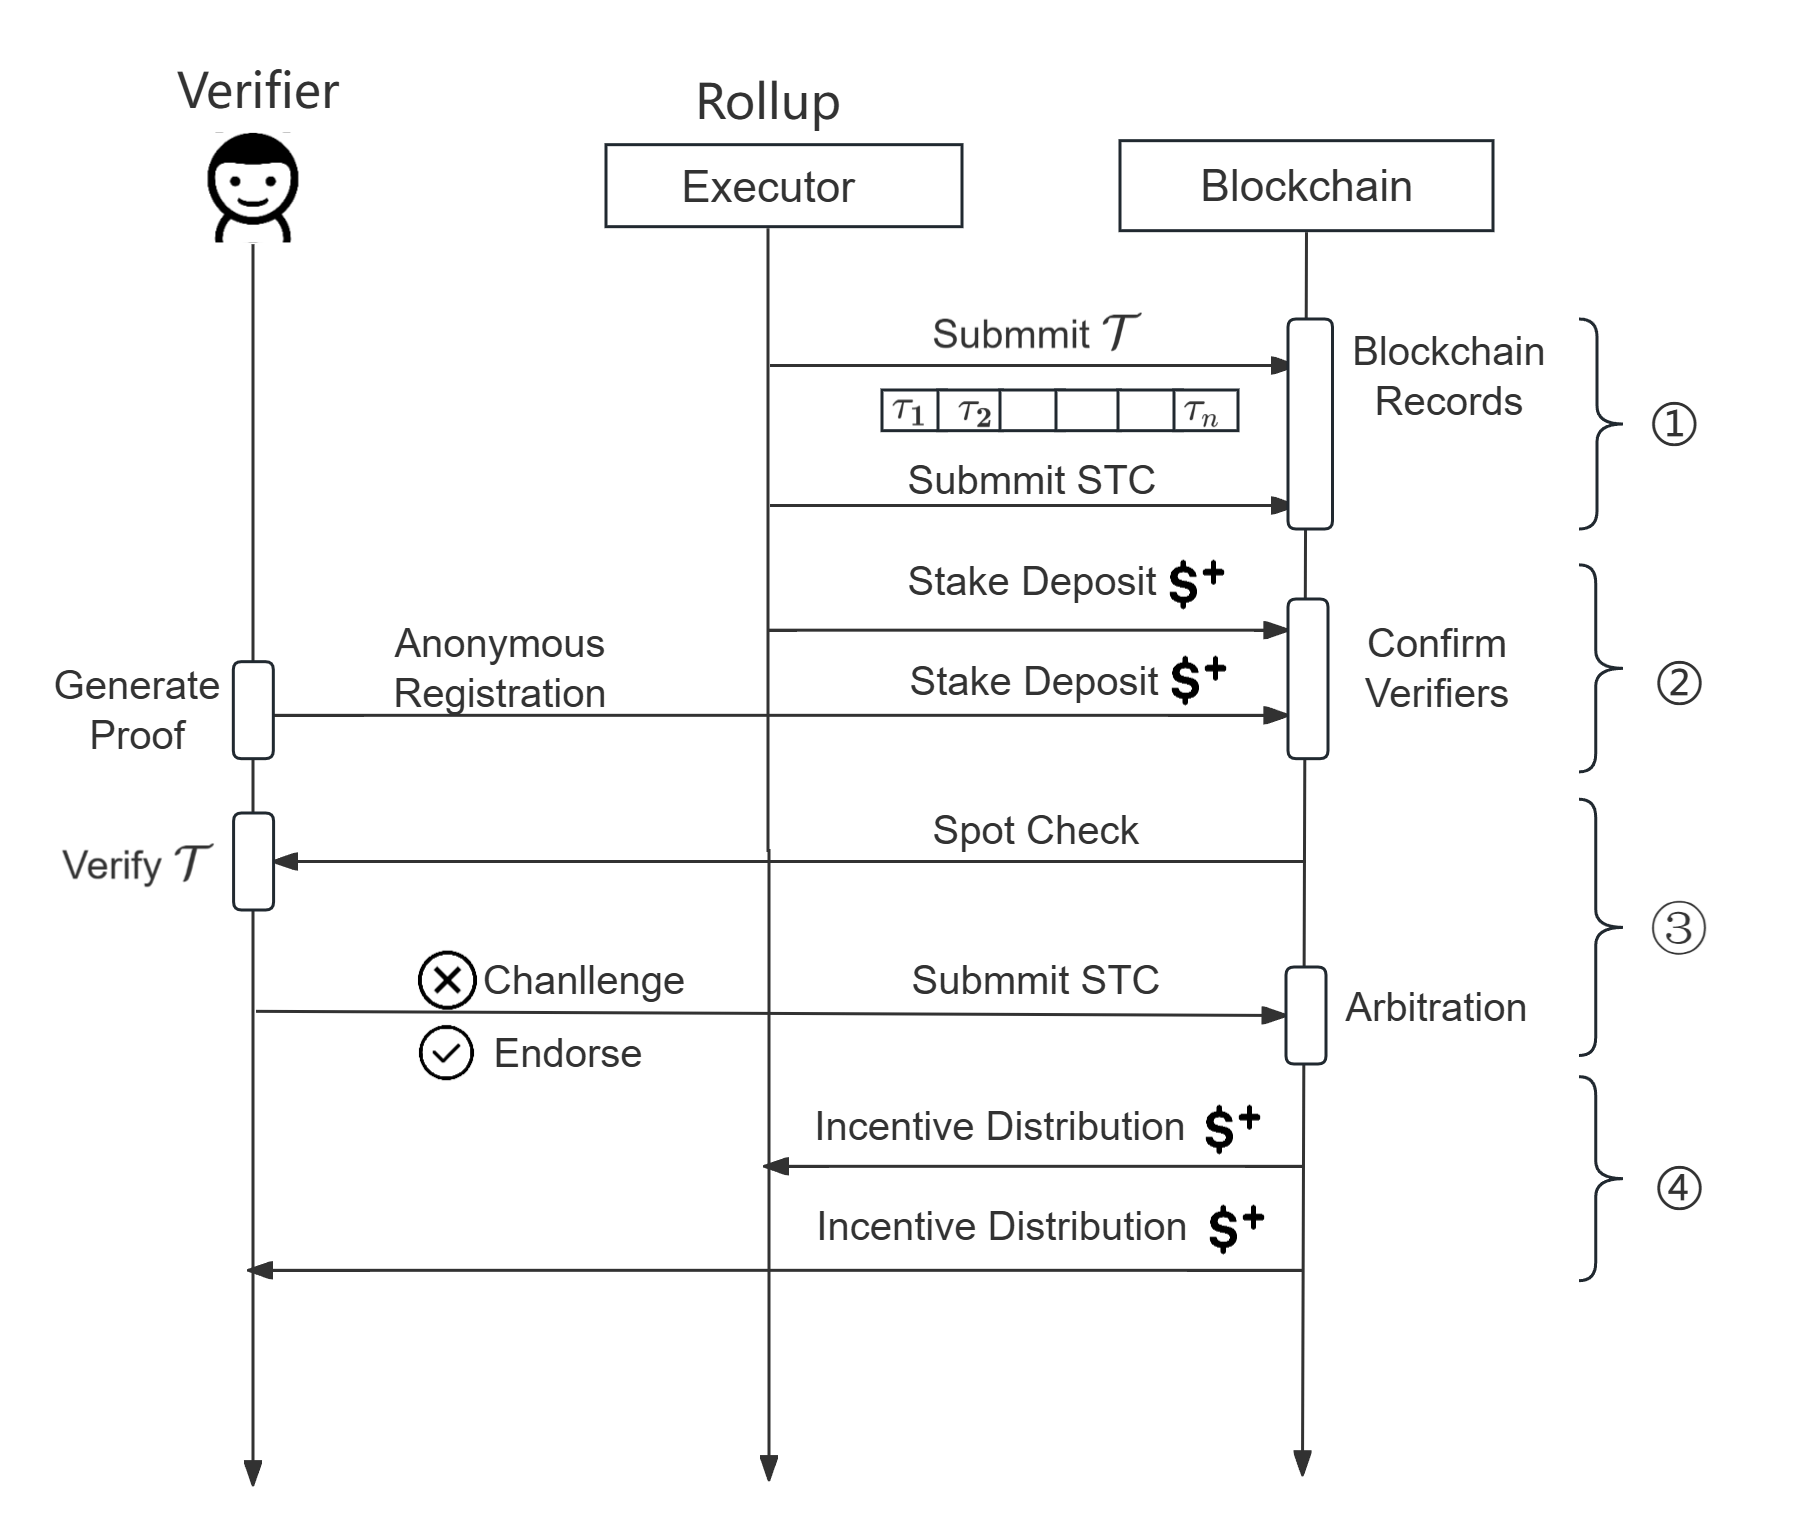
\includegraphics[width=0.7\linewidth]{Flow.png}
    \caption{AnoST Workflow}
    \label{fig:enter-label}
\end{figure}
\vspace{-15pt}

We abstract the functional modules of the blockchain-based computing verification model in Figure~\ref{fig:enter-label}, which includes three types of entities: Blockchain, Executor, Verifiers.

\begin{itemize}[noitemsep, left=0pt]

    \item \textbf{Blockchain}: The blockchain acts as the final arbitrator, handling transaction challenges initiated by verifiers, distributing incentives, and managing verifiers' anonymous identities.
    
    \item \textbf{Executor}: The executor executes transactions off-chain and submits state commitments to the blockchain for verification by verifiers.
    
    \item \textbf{Verifiers}: Verifiers independently validate transaction executions submitted by the executor, initiating on-chain challenges when discrepancies are detected to ensure authenticity and correctness.

\end{itemize}

The entire process consists of four stages，the workflow can be summarized in the following steps.

\begin{itemize}
    \item \textit{\textbf{Step 1 (Submitting Transactions):}} The executor completes the execution of the transaction set $\mathcal{T}$ off-chain and submits the corresponding state transition commitment to the blockchain, which records and stores this commitment.

    \item \textit{\textbf{Step 2 (Staking Collateral):}} Both executors and verifiers are required to stake a certain amount of collateral to the blockchain to incentivize honest participation. The blockchain deducts this collateral if dishonesty or malicious behavior is later identified.

    \item \textit{\textbf{Step 3 (Verifying Transactions):}} The system enters a verification window period, during which the blockchain randomly and anonymously schedules a set of verifiers $\mathcal{V}$ to independently verify the transaction set $\mathcal{T}$. Based on their independent verification outcomes, verifiers interact with the blockchain by either initiating explicit on-chain challenges if incorrect transactions are detected or submitting state commitments consistent with the executor.

    \item \textit{\textbf{Step 4 (Distributing Incentives):}} Upon conclusion of the verification window, the blockchain aggregates the verification results submitted by executors and verifiers, subsequently executing collateral deductions and incentive distributions accordingly, thereby incentivizing honest behaviors and penalizing dishonest actions.
\end{itemize}

\section{Anonymous Verifier Election}
This section introduces the workflow of the Anonymous Verifier Election (AVE) mechanism, a critical component ensuring system security, verifier anonymity, and protection against targeted malicious attacks.

\subsubsection{Intuition}

The AVE protocol of AnoST effectively protects verifier identity privacy. Specifically, each user registering as a verifier submits anonymous stake commitments along with verifiable anonymous identities. Verifiers register with randomized identity tags to ensure both identity confidentiality and unpredictability. When interacting with the blockchain, verifiers must provide these anonymous identity proofs along with zero-knowledge membership proofs.

After staking, the system enters the verification phase, during which verifiers generate zk-SNARK proofs to demonstrate correctness of their staked node property information. In particular, when creating anonymous stake commitments, each verifier node generates a unique identifier $C_{\text{stake}}$, concealing real identities and serving as credentials for system interactions.

To verify the correctness of staked amounts, we utilize Pedersen commitments to conceal exact staking values. Leveraging the additive homomorphic property of Pedersen commitments, we construct a balancing term $\Delta C$ to ensure value conservation. Additionally, we introduce a unique staking identifier $N_i$ to prevent double-spending attacks, thereby ensuring the uniqueness and security of each staking transaction.


\begin{figure*}[h!]

	\centering
 \small
        \fbox{
		\parbox{0.95\linewidth}{
		\vspace{-4pt}
        \begin{center}
            \textbf{Protocol} Anonymous Verification Mechanism about AnoST
            \vspace{-10pt}
        \end{center}
            
        \begin{center}
            \textbf{For each verifier $V_i$ to verify the $\mathcal{T} :\{ 
\tau_0, \tau_1, \ldots , \tau_n \} $ } 
        \end{center}

\vspace{-6pt}
$\bigstar$     \textbf{Initialization phase} \\    
% $\rhd$    $\mathsf{Setup}(1^\lambda)\rightarrow(pp,st)$ \\
$\diamond$ \textbf{System Intilize para and state}
\vspace{-8pt}
    \begin{itemize}
        \item Initialize an empty Merkle tree $\mathcal{MKT} = \{\}$ for verifier membership proofs
        \item For each $\mathcal{T}$, initialize verifier list $\mathcal{VL}_\tau = \{\}$
        \item Initialize a mapping $\mathcal{DS}_\tau = \{\}$ to prevent double-spending
        \item Select elliptic curve base points $ \mathbf{G},\ \mathbf{H} $
        % 这个验证需要质押的资金$v$
        \item set basic stake amount $v_{\text{stake}}$ about $\tau$
        \item set $\mathcal{A_\tau}$ represents the  stake address about $\mathcal{T}$
        \item call $\nizk.\keygen(1^\lambda, C_{N_i}, C_\text{mkt}, C_\text{link})\rightarrow (zpk,zvk)$
        \item set $ pp \leftarrow (\mathcal{A_\tau}, zpk, zvk, v_{\text{stake}}) $, set $st \leftarrow (\mathcal{MKT}, \mathcal{VL_\tau}, \mathcal{DS}_\tau ) $
    \end{itemize}
    
\vspace{-8pt}
$\bigstar$     \textbf{Staking and Registration phase} \\
$\diamond$ \textbf{Each verifier $V_i$ generates system parameters} 
\vspace{-8pt}
    \begin{itemize}
        \item $V_i$ get the value from anonymous mixers
        \item $ \underline{ \mathsf{AnonyReg}(1^\lambda, pp) \rightarrow (C_i, Ukey_i, \pi_{\text{mix}})} $
        \item $1 \leftarrow \nizkvf(pp, \pi_\text{mix})$, Ensure the Note $C_i$ is correct
        \item If Verification passed: $\mathcal{VL}_\tau .append(C_i)$
    \end{itemize}             
\vspace{-8pt}

$\diamond$    \textbf{Each verifier $V_i$ stakes to participate in the election}
\vspace{-8pt}
    \begin{itemize}
        % \item interpret $st$ as $(\mathcal{MKT},\mathcal{VL_\tau})$; 

        \item $\underline{ \mathsf{AnonyStake}(C_i, pp, UKey_i)  \rightarrow (\pi_{N_i}, C_{\text{change, stake, receipt}},\Delta C) } $
        
        % 防止双花攻击
        \item Check $N_i \notin \mathcal{DS_\tau}$, if it exists, exit the process directly \\
        \textcolor{mygray}{\footnotesize // \emph{In order to avoid double-spending attacks}}
        \item $ 1 \leftarrow \nizkvf(pp, \pi_{N_i}) $, If the verification fails, exit directly
        \item $\mathcal{DS_\tau}.append(N_i)$
        \item Check $ C_i + \Delta C == C_{\text{stake}} + C_{\text{change}} $ or $C_i == C_{\text{stake}} + C_{\text{change}} + \Delta C $ \\
        \textcolor{mygray}{\footnotesize // \emph{Checking the conservation of amount}}

        \item Check $C_{\text{stake}} == C_{receipt} + v_{stake} \mathbf{H}$

        \item The pledged funds are deposited into the system fund pool
        \item $\mathcal{VL}_\tau.append(C_{\text{stake}})$, Regard the $C_{\text{stake}}$ as new $C_i$
    \end{itemize}
\vspace{-8pt}
    
$\bigstar$     \textbf{Verification and Scheduling phase} \\   
$\diamond$    \textbf{Schedule verifiers to verify computation tasks $\tau$ }   
\vspace{-8pt}
    \begin{itemize}
        \item Sample $R$ from random beacon, set R as the verifier number
        \item $\mathcal{VL}_\tau' \leftarrow Filter(\mathcal{VL}_\tau, R)$ , Compute Merkle tree commiment as $\mathcal{H}_{root}$
    \end{itemize}

\vspace{-8pt}
$\diamond$ \textbf{For each verifier $V_i$ in $\mathcal{VL}_\tau'$ to verify tasks $\tau$ }
\vspace{-8pt}
    \begin{itemize}
        \item $\underline{  \mathsf{Endorse} (pp, st, C_{\text{stake}}, \mathcal{H}_{root}) \rightarrow Res }$
        \item Authenticate the identity of anonymous verifiers
        \item Parse evidence parameter $Res.\pi$ as $ (\pi_{path}, \pi_{link})$
        \item Verify merkle-tree path: $1 \leftarrow \nizkvf(pp, \pi_{path})$
        \item Verify linkability proof: $ 1 \leftarrow \nizkvf(pp, \pi_{link}) $
        \item Output 1 if and only if the above conditions is true
        \item Otherwise, output 0 \textcolor{mygray}
    {\footnotesize // \emph{The authentication is incorrect}}
    \end{itemize}
\vspace{-8pt}
            }
	 }
	\caption{Anonymous Verification Election Mechanism AVE} 
        \vspace{-15pt}
	\label{AVE}
\end{figure*}

\subsubsection{Construction}

The AVE protocol is illustrated in Fig.~\ref{AVE}, where the underlined segments indicate specific implementation actions performed by each verifier. These actions will be elaborated in detail in the subsequent section. The AVE protocol comprises the following stages:

\begin{itemize}
    \item \textbf{Initialization Phase}: The system is first initialized, establishing public data structures and public parameters. Participating verifiers then generate their associated cryptographic keys.

    \item \textbf{Staking and Registration Phase}: Verifier nodes intending to participate in anonymous staking apply to join the verification system. During the anonymous staking and registration process, an identity identifier is generated. Successfully staked nodes are then aggregated into a global verifier list, from which verifiers are selected.

    \item \textbf{Verification Phase}: The system assigns a group of verifiers to each task. Assigned verifiers independently perform transaction verification. If discrepancies are detected, verifiers initiate an on-chain challenge. Based on the verification outcomes, the blockchain subsequently enforces rewards and penalties for the involved parties.
\end{itemize}


\subsection{Protocol and verifiers interaction details}

The AVE protocol describes the overall process of anonymous verification of tasks. Next, we will give a detailed description of the key functions involved.

\vspace{-8pt}

\[
\underline{ \mathsf{AnonyReg}(1^\lambda, pp) \rightarrow (C_i, Ukey_i, \pi_{\text{mix}})  }
\]

In the anonymous registration phase, each verifier needs to complete key generation, anonymous recharge, and system registration.


\begin{enumerate}[label=(\arabic*)]

    \item \textbf{Key Generation.}  
    New verifiers are required to complete identity registration before joining the system. Each verifier generates a personal key pair and a random scalar $r_i$, which is used to construct a Pedersen commitment and also serves as part of the verifier’s identity.
    
    \item \textbf{Anonymous Registration.}  
    To prevent Sybil attacks, the system requires verifiers to deposit a certain amount of funds before they can participate. Verifiers anonymously deposit their funds into the system via a mixer, which breaks the traceability between the fund source and the verifier’s identity. During this process, the verifier generates a commitment $C_i = r_i \mathbf{G} + v_i \mathbf{H} $ along with a zero-knowledge proof of the committed amount $ \pi_\text{mix} = \nizk(\exists{v_i = \text{mix amount} },  \text{s.t.}\ C_i = r_i \mathbf{G} + v_i \mathbf{H} ) $. Upon successful verification, $C_i$ is bound to verifier $V_i$ as their identity representation.
    
\end{enumerate}

\vspace{-15pt}

\[
\underline{ \mathsf{AnonyStake}(C_i, pp, UKey_i)  \rightarrow (\pi_{N_i}, C_{\text{change, stake}}, \Delta C)  }
\]

\begin{enumerate}[label=(\arabic*)]

    \item \textbf{Stake Preparation.}  
    Verifier selects input note $ C_i $, which representing the current balance and identity state. Based on the staking parameters, they compute two new output notes: the staking note $ C_{\text{stake}} = r_{\text{stake}} \mathbf{G} + v_{\text{stake}} \mathbf{H} $ and the change note $C_{\text{change}} = r_{\text{change}} \mathbf{G} + v_{\text{change}} \mathbf{H}$, ensuring value conservation and uniqueness of the commitments.
    
    \item \textbf{Proof Generation.}  
    The verifier first computes the nullifier to prevent double-spending $ N_i = \hash_1(r_i, C_i, index) $. Then, a zero-knowledge proof $\pi_{N_i} = \nizk(\exists r_i\ \text{s.t.}\  N_i = \hash_1(r_i, C_i, index(C_i)))$ is generated to prove ownership of the input note \( C_i \) and the correctness of the output amounts without revealing any sensitive information.
    
    \item \textbf{Staking and Broadcasting.}  
    The prover packages the transaction and broadcasts it to the blockchain. The transaction includes the stake note $C_\text{stake}$, change note $C_\text{change}$, the nullifier \( N_i \), and the corresponding zero-knowledge proof \( \pi_{N_i} \), ensuring both transaction validity and anonymity. At the same time, a balance item $\Delta C = r'\mathbf{G}$ is calculated to verify the correctness of the pledge.
    
    \item \textbf{Verification and State Update.}  
    The system verifies the validity of the zero-knowledge proof and checks whether the nullifier \( N_i \) has been used before. If valid, the staking note is accepted as locked capital, and the system state is updated accordingly.

\end{enumerate}

In summary, the verifier anonymously stakes assets by splitting an input note $C_i$ into a staking note $C_{\text{stake}}$ and a change note $C_{\text{change}}$. A nullifier $N_i$ and zero-knowledge proof are generated to ensure correctness and prevent double-spending without revealing private information.

\vspace{-6pt}

\[
\underline{  \mathsf{Endorse} (pp, st, C_{\text{stake}}, \mathcal{H}_{root}) \rightarrow Res }
\]

\begin{enumerate}[label=(\arabic*)]
    \item \textbf{Identity Proof Generation.} Verifiers generate a Merkle-tree existence proof $\pi_{path}$ to ensure that only authorized verifiers can participate in verifying the computational task. Subsequently, verifiers produce a linkability proof $ \pi_{link} = \nizk\{ \exists r_{stake}, \ \text{s.t.} \  C_{stake} = r_{stake} \mathbf{G} + v_{stake} \mathbf{H} \} $ to confirm that the current \( C_{stake} \) was indeed created by themselves. This process effectively prevents impersonation while preserving verifiers' anonymity.
    
    \item \textbf{Task Verification.} Upon receiving a task requiring verification, verifiers immediately initiate an on-chain challenge if they detect any incorrect transactions within the task. The correctness of the challenged transaction is subsequently determined on-chain.
    

\end{enumerate}  

\subsection{Protocol Correctness Explanation}

\textbf{Anonymity Explanation.}  During the execution of the protocol, each verifier generates an identity commitment $C_i$ using a Pedersen commitment, which serves as their anonymous identity tag. At the same time, a network relay is used during blockchain interactions to hide the source address of transactions. When submitting verification results, the verifier uses a zk-SNARK to prove knowledge of the corresponding random scalar $r_i$, thereby achieving identity linkage. Throughout the entire protocol, no real-world identity information of the verifier is ever exposed.

\textbf{Staking Correctness Explanation.}  Verifiers participate in the election by staking funds. According to the principle of value conservation, we have $v_{\text{change}} = v_i + v_{\text{stake}}$. Meanwhile, the verifier computes a balancing term $\Delta C$ to ensure that the randomness in the commitments is not reduced. The system verifies the following equation based on the additive homomorphism of Pedersen commitments:

\[
C_i + \Delta C = C_{\text{stake}} + C_{\text{change}}
\]

This can be further expanded as:

\[
(r_i + r')\mathbf{G} + v_i \mathbf{H} = (r_{\text{stake}} + r_{\text{change}}) \mathbf{G} + (v_{\text{stake}} + v_{\text{change}}) \mathbf{H}
\]

To prevent double-spending attacks, each verifier must submit a proof $N_i$ bound to their identity and $C_i$ before initiating a transaction. The system checks for the existence of $N_i$ to ensure it has not been reused.

\section{Commitment and Challenge Verification}

In this section, we introduced the State Transition Commitment (STC) mechanism, which effectively verifies verifiers' workloads and addresses the verifier's dilemma. Furthermore, based on the State Transition Tree (STT), we proposed a refined challenge and pruning mechanism, enabling precise rollback of erroneous transactions and efficient confirmation of valid ones, significantly enhancing system verification performance.

\subsection{Overview}
Optimistic verification security heavily relies on verifiers actively checking off-chain transactions. However, since executors typically submit correct transactions due to strict staking penalties, rational verifiers may avoid costly verification, adopting a strategy called \textit{free-riding}. This behavior, termed the \textit{Verifier's Dilemma}, can severely undermine security if incorrect transactions escape detection.

To resolve this, we propose a \textit{State Transition Commitment (STC)} mechanism based on a \textit{State Transition Tree (STT)}—a DAG structure explicitly recording transaction state transitions. Executors and verifiers independently compute and submit state transition commitment hashes along with random seeds to the blockchain. Commitment consistency is efficiently verified through hash comparison without costly on-chain re-execution, addressing the verifier's dilemma.

\textbf{Intuition:}
The dilemma occurs because blockchains economically cannot verify whether verifiers genuinely performed validations. Our STC mechanism requires verifiers explicitly record transaction input-output states, providing verifiable proof of their verification work.

Specifically, executors first submit an STC hash and random seed. During the verification window, verifiers independently validate transactions, submitting their own STC hashes and seeds, and initiating on-chain challenges if discrepancies occur. After revealing seeds, the blockchain resolves inconsistencies; otherwise, the batch is confirmed correct. This ensures genuine verifier participation.

Based on the \textbf{Anonymous Verifier Election} mechanism, we assume verifiers independently verify transactions without collusion, ensuring objectivity and simplifying consistency checks.

Thus, the STC framework explicitly records input-output states as execution commitments on-chain, significantly reducing verification overhead. The detailed mechanism is presented subsequently.

\subsection{Mechanism Design and Workflow Description}
To clearly illustrate the detailed execution process of the STC mechanism, this section elaborates on constructing the State Transition Tree (STT) and the corresponding on-chain verification procedure. Specifically, the STC mechanism precisely records off-chain transaction state changes and employs efficient hash-consistency verification on-chain, significantly reducing verification costs while ensuring transaction correctness.

The STC mechanism comprises three stages: (1) STT construction, (2) independent verifier commitments, and (3) on-chain hash verification and challenges.

\begin{itemize}
    \item \textbf{Stage 1: STT Construction}  

    The off-chain executor strictly records input-output states for each transaction in the batch awaiting verification, specifying dependencies and execution order. After executing all transactions, the executor constructs a complete State Transition Tree ($\mathcal{T}_{\text{exec}}$), comprising \textit{State Nodes} and \textit{Transaction Nodes}.  

    Each \textit{State Node} records the resulting state after transaction execution, defined as:
    \[
    H(S_i) = \mathcal{H}(S_i^{\text{data}})
    \]

    Each \textit{Transaction Node} represents individual transaction execution, containing detailed transaction data (e.g., function calls, parameters), explicitly linking input and output state nodes. Its hash is defined as:
    \[
    H(\tau_i) = \mathcal{H}(\tau_i \parallel H(S_i^{\text{in}}) \parallel H(S_i^{\text{out}}))
    \]

    Here, $\tau_j$ ensures transaction uniqueness (e.g., transaction signature or hash of the content itself), enabling explicit identification and verification. All nodes collectively form a DAG, constituting the STT. The executor then calculates node hashes from bottom-up, obtaining the STT root hash ($h_{\text{exec}} = \mathcal{R_H}(\mathcal{T}_{\text{exec}})$), submitted to the on-chain smart contract.

    \item \textbf{Stage 2: Independent Verifier Commitments}  

    During the verification window, each verifier independently executes off-chain verification tasks to confirm transaction correctness. Each verifier constructs its own STT ($\mathcal{T}_{v_i}$) following the same method as the executor, calculates hashes for nodes, and submits the resulting root hash to the blockchain:
    \[
    h_{v_i} = \mathcal{R_H}(\mathcal{T}_{v_i})
    \]

    Independent root hash submissions explicitly demonstrate verifiers' verification effort, deterring cheating.

    \item \textbf{Stage 3: On-chain Hash Verification and Challenges}  

    After the verification window, the on-chain smart contract automatically checks the consistency of STT root hashes submitted by executors and verifiers. If verifier hashes match the executor’s hash (i.e., $h_{v_i} = h_{\text{exec}}$), transaction correctness is confirmed without further action. Discrepancies indicate potential transaction errors, triggering an on-chain challenge resolution process. Detailed challenge handling is elaborated in the next section.
\end{itemize}



\subsection{State Pruning and Partial Transaction Confirmation}

Traditional optimistic verification mechanisms typically reject an entire transaction batch upon detecting any single erroneous transaction, significantly limiting transaction acceptance rates. To address this, we propose a \textit{state pruning and partial transaction confirmation mechanism} based on the State Transition Tree (STT), allowing selective rollback of erroneous transactions without impacting correct transactions.

Specifically, after the verification window period, the blockchain checks the consistency of STT root hashes submitted by verifiers and executors. If the root hashes match (i.e., $h_{v_i}=h_{\text{exec}}$), the batch correctness is confirmed. If discrepancies arise, indicating potential erroneous transactions, a verifier submits a path proof $\pi(\tau_k)$ targeting the disputed transaction node $\tau_k$. This proof includes hashes along the path from the STT root node to the challenged node, together with sibling nodes at each layer.

Upon receiving the proof, the on-chain smart contract reconstructs the root hash from the challenged node upwards. If the reconstructed root hash matches the executor's submitted root hash, the verifier's challenge is invalid, resulting in stake forfeiture. If not, the executor is confirmed malicious, and the verifier receives the executor's stake as compensation.

Once transaction $\tau_k$ is confirmed erroneous, the smart contract initiates the state pruning procedure, removing $\tau_k$ and all subsequent dependent nodes from the executor's STT ($\mathcal{T}_{\text{exec}}$). It then recalculates hashes from bottom to top, deriving a new, valid STT root hash $h_{\text{exec}}'$.

The updated root hash $h_{\text{exec}}'$ is publicly announced, ensuring all off-chain nodes quickly synchronize to the latest correct state. Our refined on-chain challenge and pruning mechanism selectively rolls back only erroneous transactions, enabling unaffected transactions to be smoothly validated and confirmed. This significantly improves transaction throughput, reduces on-chain validation and storage overhead, and enhances overall system performance and scalability.


\subsection{Protocol Correctness Analysis}

We now rigorously analyze the correctness and verifiability of the proposed protocol based on previously defined notations and concepts. Given a transaction batch $\mathcal{T}=\{\tau_i\}_{i=1}^{n}$, the executor constructs the corresponding State Transition Tree $\mathcal{T}_{\text{exec}}$, submitting its root hash commitment $h_{\text{exec}}=\mathcal{R_H}(\mathcal{T}_{\text{exec}})$ to the blockchain. Each verifier $v_i$ independently verifies the transaction batch $\mathcal{T}$, constructing their own State Transition Tree $\mathcal{T}_{v_i}$ and submitting the root hash $h_{v_i}=\mathcal{R_H}(\mathcal{T}_{v_i})$.

As defined previously, the hash of each transaction node explicitly depends on its input and output state node hashes:
\[
H(\tau_j) = \mathcal{H}(\tau_j \parallel H(S_j^{\text{in}}) \parallel H(S_j^{\text{out}})),
\]
while each state node directly encodes the post-execution state data:
\[
H(S_j) = \mathcal{H}(S_j^{\text{data}}).
\]

Thus, verifiers must genuinely verify each transaction $\tau_j \in \mathcal{T}$ to correctly derive intermediate states $S_j^{\text{data}}$ and compute a consistent root hash $h_{v_i}$. Failure to perform complete verification inevitably leads to discrepancies between the verifier’s root hash and the executor's commitment, efficiently detectable during on-chain consistency checks. Formally:
\[
h_{v_i} \neq h_{\text{exec}} \quad \Longleftrightarrow \quad \exists \tau_j, S_j^{\text{in}}, S_j^{\text{out}}, (S_j^{\text{in}}, \tau_j, S_j^{\text{out}}) \notin \mathcal{T}_{v_i}.
\]

Additionally, our experimental section introduced a \textit{path-inclusion detection mechanism} to further ensure accurate and efficient on-chain challenges. Specifically, transaction batches may contain multiple dependent transaction paths. When a verifier successfully challenges a transaction $\tau_x$ within a path $\mathcal{P}(\tau_x)=\{\tau_1,\dots,\tau_x,\dots,\tau_m\}$, all subsequent dependent transactions ($\tau_y$, where $x<y \leq m$) on that path are automatically invalidated. Formally, we denote this property as:
\[
\forall \tau_x, \tau_y \in \mathcal{P}, x<y,\quad \tau_y \text{ is invalidated.}
\]

This means subsequent challenges targeting transactions following an already successfully challenged transaction in the same path will be ignored by the blockchain, preventing redundant verification efforts.

The correctness of this path detection mechanism inherently leverages the STT structure: each transaction node explicitly depends on the output state of its preceding node. Hence, if a preceding node $\tau_x$ is identified as erroneous, the output states of subsequent nodes ($\tau_y$ with $y>x$) become invalid by definition. Consequently, straightforward on-chain path detection effectively prevents redundant challenges, significantly reducing verification overhead and improving challenge efficiency.

Finally, the anonymous verifier election mechanism introduced earlier inherently restricts effective communication among verifiers, fundamentally preventing collusion risks. Consequently, our mechanism explicitly ensures verifiers' workload verifiability, completely eliminating incentives and possibilities for free-riding or lazy verification, significantly enhancing the security, correctness, and efficiency of the system even under malicious conditions.

\section{Security Analysis}
In this section, we rigorously analyze the security properties of AnoST, focusing on three essential guarantees: verifier anonymity, anti-collusion (workload verifiability), and game-theoretic resolution of the Verifier's Dilemma.

\subsection{Verifier Anonymity}
\begin{definition}[Verifier Anonymity]
Let $\mathcal{A}$ denote a probabilistic polynomial-time adversary. We define verifier anonymity via the following indistinguishability game:
\begin{enumerate}
    \item The challenger chooses random commitments $(C_0, C_1)$, corresponding to distinct verifiers $(V_0,V_1)$ with commitments $C_i = r_i \mathbf{G} + v \mathbf{H}$.
    \item The challenger samples a random bit $b \xleftarrow{\$} \{0,1\}$ and provides $C_b$ to $\mathcal{A}$.
    \item Adversary $\mathcal{A}$ outputs a guess $b' \in \{0,1\}$.
\end{enumerate}
AnoST achieves verifier anonymity if for all PPT adversaries $\mathcal{A}$,
\[
\left| \Pr[b' = b] - \frac{1}{2} \right| \leq \text{negl}(\lambda)
\]
where $\lambda$ is the security parameter.
\end{definition}

\begin{theorem}[Verifier Anonymity]
AnoST guarantees verifier anonymity under the hardness assumption of the elliptic curve discrete logarithm problem (ECDLP).
\end{theorem}

\begin{proof}
Verifier anonymity in AnoST fundamentally relies on the Pedersen commitment $C = r\mathbf{G} + v \mathbf{H}$, which is known to provide unconditional hiding. To break anonymity, adversary $\mathcal{A}$ must distinguish between two commitments. Since commitments are perfectly hiding and independent of verifier identity, distinguishing $C_0$ from $C_1$ requires the adversary to compute $r_i$ given $C_i$, thus solving the discrete logarithm of elliptic curve group $\mathbb{G}$. Given ECDLP is computationally infeasible, the adversary's advantage must remain negligible. Hence, AnoST preserves verifier anonymity.
\end{proof}

\subsection{Anti-collusion: Workload Verifiability}
\begin{definition}[Workload Verifiability]
Consider a transaction set $T = \{\tau_i\}_{i=1}^{n}$, where each verifier $V_j$ independently computes a State Transition Tree (STT) $T_{V_j}$ with root hash $h_{V_j}$. The system ensures workload verifiability if:
\[
h_{V_j} = RH(T_{\text{exec}}) \iff \forall \tau_i \in T, V_j \text{ executed } \tau_i \text{ correctly}
\]
\end{definition}

\begin{theorem}[Workload Verifiability]
AnoST achieves workload verifiability assuming collision-resistance and pre-image resistance of the cryptographic hash function.
\end{theorem}

\begin{proof}
To generate a valid STT root hash $h_{V_j}$ identical to the executor's $h_{\text{exec}}$, a verifier $V_j$ must correctly compute every intermediate state $S_i^{out}$ for each transaction $\tau_i \in T$. The STT node hashes are computed as follows:
\[
H(\tau_i) = H(\tau_i \| H(S_i^{in}) \| H(S_i^{out}))
\]
If a verifier attempts to bypass actual computation, it must guess or reproduce the exact output state $S_i^{out}$ for each transaction. Given the pre-image resistance and collision-resistance of the hash function, the probability of correctly guessing these outputs without actual computation is negligible. Consequently, generating a consistent $h_{V_j}$ without full verification is computationally infeasible. Thus, AnoST guarantees workload verifiability.
\end{proof}

\subsection{Resolution of the Verifier's Dilemma}
To demonstrate AnoST's resolution of the Verifier's Dilemma, we construct a game-theoretic model to analyze verifier incentives.

\begin{definition}[Verifier Game]
We define a strategic game $G = (V, \{S_i\}, \{u_i\})$, where:
\begin{itemize}
    \item $V = \{V_1,\dots,V_n\}$ is the set of verifiers.
    \item Each verifier $V_i$ selects a strategy $s_i \in S_i = \{\textsf{Verify}, \textsf{Skip}\}$.
    \item Payoff function $u_i: S \to \mathbb{R}$ is defined as follows:
    \begin{itemize}
        \item $u_i(\textsf{Verify}) = r - c$, where $r$ is the verification reward, and $c$ is the verification cost.
        \item $u_i(\textsf{Skip}) = r - P_{detect}\cdot p$, where $p$ is the penalty if the skipping is detected and $P_{detect}$ is the detection probability.
    \end{itemize}
\end{itemize}
\end{definition}

\begin{theorem}[Verifier's Dilemma Resolution]
If the system parameters satisfy $P_{detect}\cdot p > c$, then $\textsf{Verify}$ is the strictly dominant strategy, and AnoST resolves the Verifier's Dilemma.
\end{theorem}

\begin{proof}
To prove this, we calculate the expected payoffs explicitly. A verifier selecting $\textsf{Skip}$ obtains an expected payoff:
\[
\mathbb{E}[u_i(\textsf{Skip})] = r - P_{detect}\cdot p
\]
A verifier selecting $\textsf{Verify}$ has a deterministic payoff:
\[
u_i(\textsf{Verify}) = r - c
\]
The rational verifier will choose $\textsf{Verify}$ if and only if:
\[
r - c > r - P_{detect}\cdot p \quad \Rightarrow \quad P_{detect}\cdot p > c
\]
Thus, under the given incentive parameters, the dominant strategy equilibrium is all verifiers performing verification. Consequently, AnoST economically enforces honest verification and resolves the Verifier's Dilemma.
\end{proof}

Through this rigorous analysis, we demonstrate that AnoST provides robust security guarantees, ensuring verifier anonymity, effective workload verifiability, and economically-driven resolution of the Verifier's Dilemma.


\section{Implementation}
The primary evaluation objective of AnoST is to demonstrate its core benefits in precise rollback capabilities, verifier anonymity protection, and the resolution of the Verifier’s Dilemma. Our experiments are structured around verifying these security and mechanism effectiveness goals, rather than maximizing general performance metrics such as transaction throughput.

We benchmarked the circuit compilation and proof generation overhead of AnoST’s zero-knowledge circuits ($\pi_{\text{mix}}, \pi_{N_i}, \pi_{link}$) using an Intel i5-12400H CPU with 32GB RAM, Circom, and snarkJS. Proofs were generated in a single-threaded environment. On-chain verification times were measured on a blockchain simulation node (AMD EPYC 7302P, 64GB RAM). Results summarized in Table~\ref{table:zk-overhead} confirm that the computational overhead is moderate, demonstrating practical deployability.

% \vspace{-1em}
\begin{table}[h]
\centering
\caption{Zero-Knowledge Proof Performance Overhead}
\label{table:zk-overhead}
\begin{tabular}{p{8em} p{8em} p{8em} p{6em}}
\toprule
\textbf{Proof Task} & \textbf{Gen Time} & \textbf{Prove Time} & \textbf{Set Time} \\
\midrule
$\pi_\text{mix}$ & 297ms & 2.4ms & 1.2s \\
$\pi_{N_i}$ & 1.43s & 1.3s & 5.2s \\
$\pi_{link}$ & 286ms & 2.3ms & 1.1s \\
\bottomrule
\end{tabular}
\end{table}

We evaluated AnoST’s on-chain gas consumption in the Ethereum Virtual Machine (EVM) environment. Figure~\ref{fig:gascost} presents the gas costs breakdown for verifier committee election without zero-knowledge aggregation, scaling the number of verifiers from 50 to 200. Our results illustrate that AnoST maintains efficient on-chain execution costs, approximately 0.005\$ per execution on Binance Smart Chain (BSC) and 0.0024\$ on Polygon, highlighting its economic feasibility.

\begin{figure}[h]
\centering
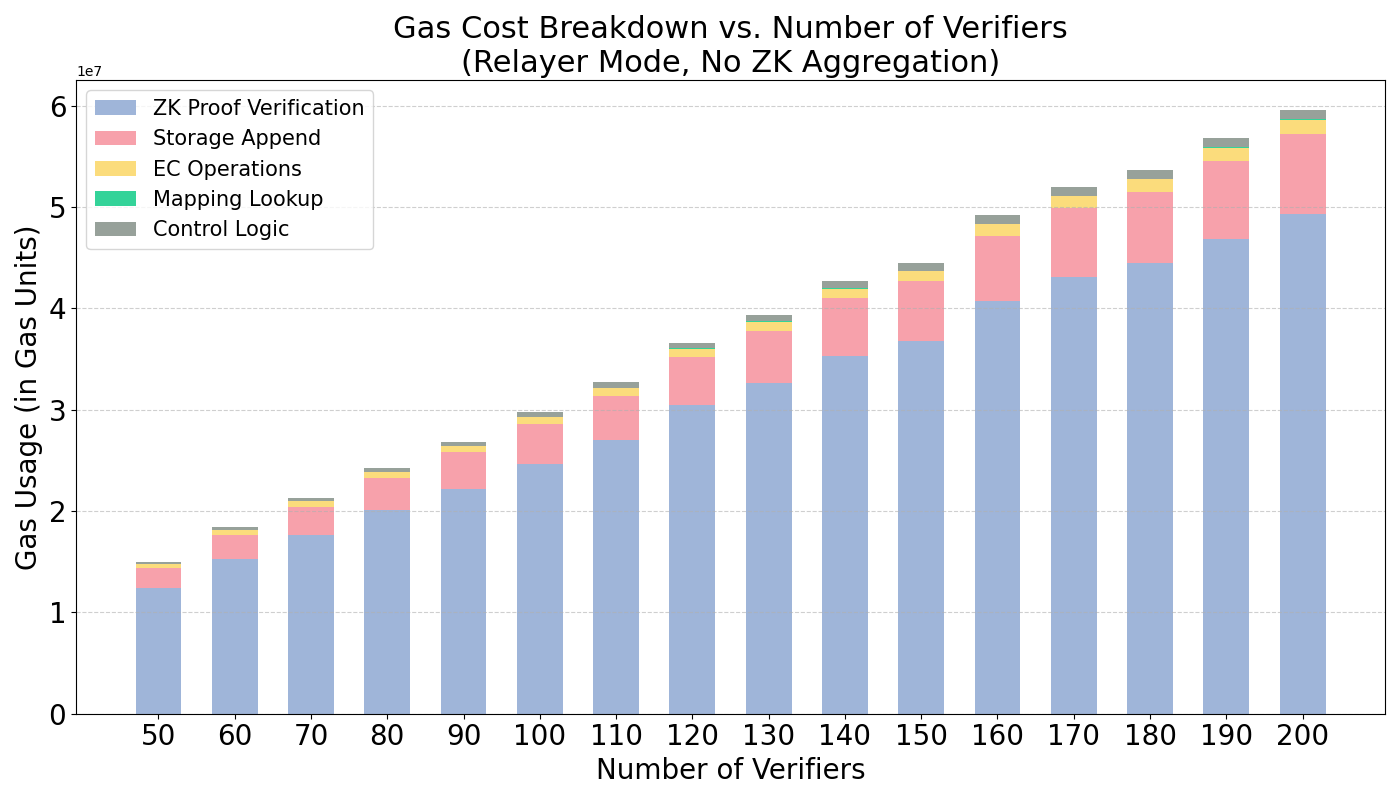
\includegraphics[width=0.8\linewidth]{GasCost.png}
\caption{AnoST Committee Election Gas Cost On Chain}
\label{fig:gascost}
\end{figure}

To evaluate the effectiveness of the State Transition Tree (STT) mechanism, we implemented a deterministic local simulator following the DAG construction, path-inclusion detection, and pruning rules described above. Each trial contains 2000 transactions assigned to 600 dependency paths, and each error-ratio setting is averaged over 50 independently generated batches. Table~\ref{tab:rollback-experiment-new} summarizes local STT construction time, compact off-chain storage overhead, rollback settlement time, and transaction pass rate.

\begin{table}[h!]
\centering
\caption{STT Partial Rollback Performance}
\label{tab:rollback-experiment-new}
\renewcommand{\arraystretch}{1}
\begin{tabular}{ccccc}
\toprule
Error Ratio (\%) & Build STT (s) & Storage Cost (KB) & Rollback Time (s) & Pass Rate (\%) \\
\midrule
0  & 0.0055 & 281.2 & 0.00 & 100.0 \\
5  & 0.0055 & 281.2 & 0.91 & 89.5 \\
10 & 0.0055 & 281.2 & 1.56 & 79.6 \\
15 & 0.0055 & 281.2 & 2.12 & 70.9 \\
20 & 0.0055 & 281.2 & 2.63 & 62.8 \\
\bottomrule
\end{tabular}
\end{table}

The results show that STT construction remains lightweight for 2000-transaction batches, averaging about 5.5 ms in the local simulator. As the error ratio rises, rollback time increases because more dependency paths must be settled, but the mechanism still preserves 62.8\% of transactions at a 20\% error ratio; a full-batch rollback baseline would accept 0\% once any erroneous transaction appears.

To further validate that the rollback procedure can be demonstrated in a real execution environment, we implemented a minimal STT rollback smart contract and executed it on a local Anvil EVM node using Foundry. The contract commits an STT root, accepts path-level challenge proofs, records pruned paths, and settles the remaining accepted transactions. Table~\ref{tab:evm-rollback-demo} reports the wall-clock time and gas consumption measured from actual RPC transactions.

\begin{table}[h!]
\centering
\caption{Local EVM STT Rollback Demo}
\label{tab:evm-rollback-demo}
\renewcommand{\arraystretch}{1}
\begin{tabular}{cccccc}
\toprule
Error Ratio (\%) & Challenge Paths & Invalidated TXs & Pass Rate (\%) & EVM Time (s) & Total Gas \\
\midrule
5  & 5  & 210 & 89.5 & 6.96  & 585650 \\
10 & 8  & 409 & 79.5 & 9.95  & 798590 \\
20 & 10 & 745 & 62.7 & 11.87 & 951930 \\
\bottomrule
\end{tabular}
\end{table}

The local EVM run completes all three demonstration settings in under 30 seconds excluding one-time compilation, while each individual error-ratio setting completes in less than 12 seconds. This provides a practical demonstration path for the STT rollback logic without relying solely on the deterministic simulator.

We further evaluated challenge-window duration in seconds using the same 50-batch simulation setting, testing 5\%, 10\%, and 20\% transaction error ratios. Four defensive mechanisms were evaluated: (1) No Optimization, (2) Path Checking, which skips redundant challenges whose dependency suffix has already been invalidated, (3) Blacklist, which blocks previously detected malicious verifiers after a setup cost, and (4) Combined Optimization, which applies both mechanisms.

\begin{figure}[h!]
\centering
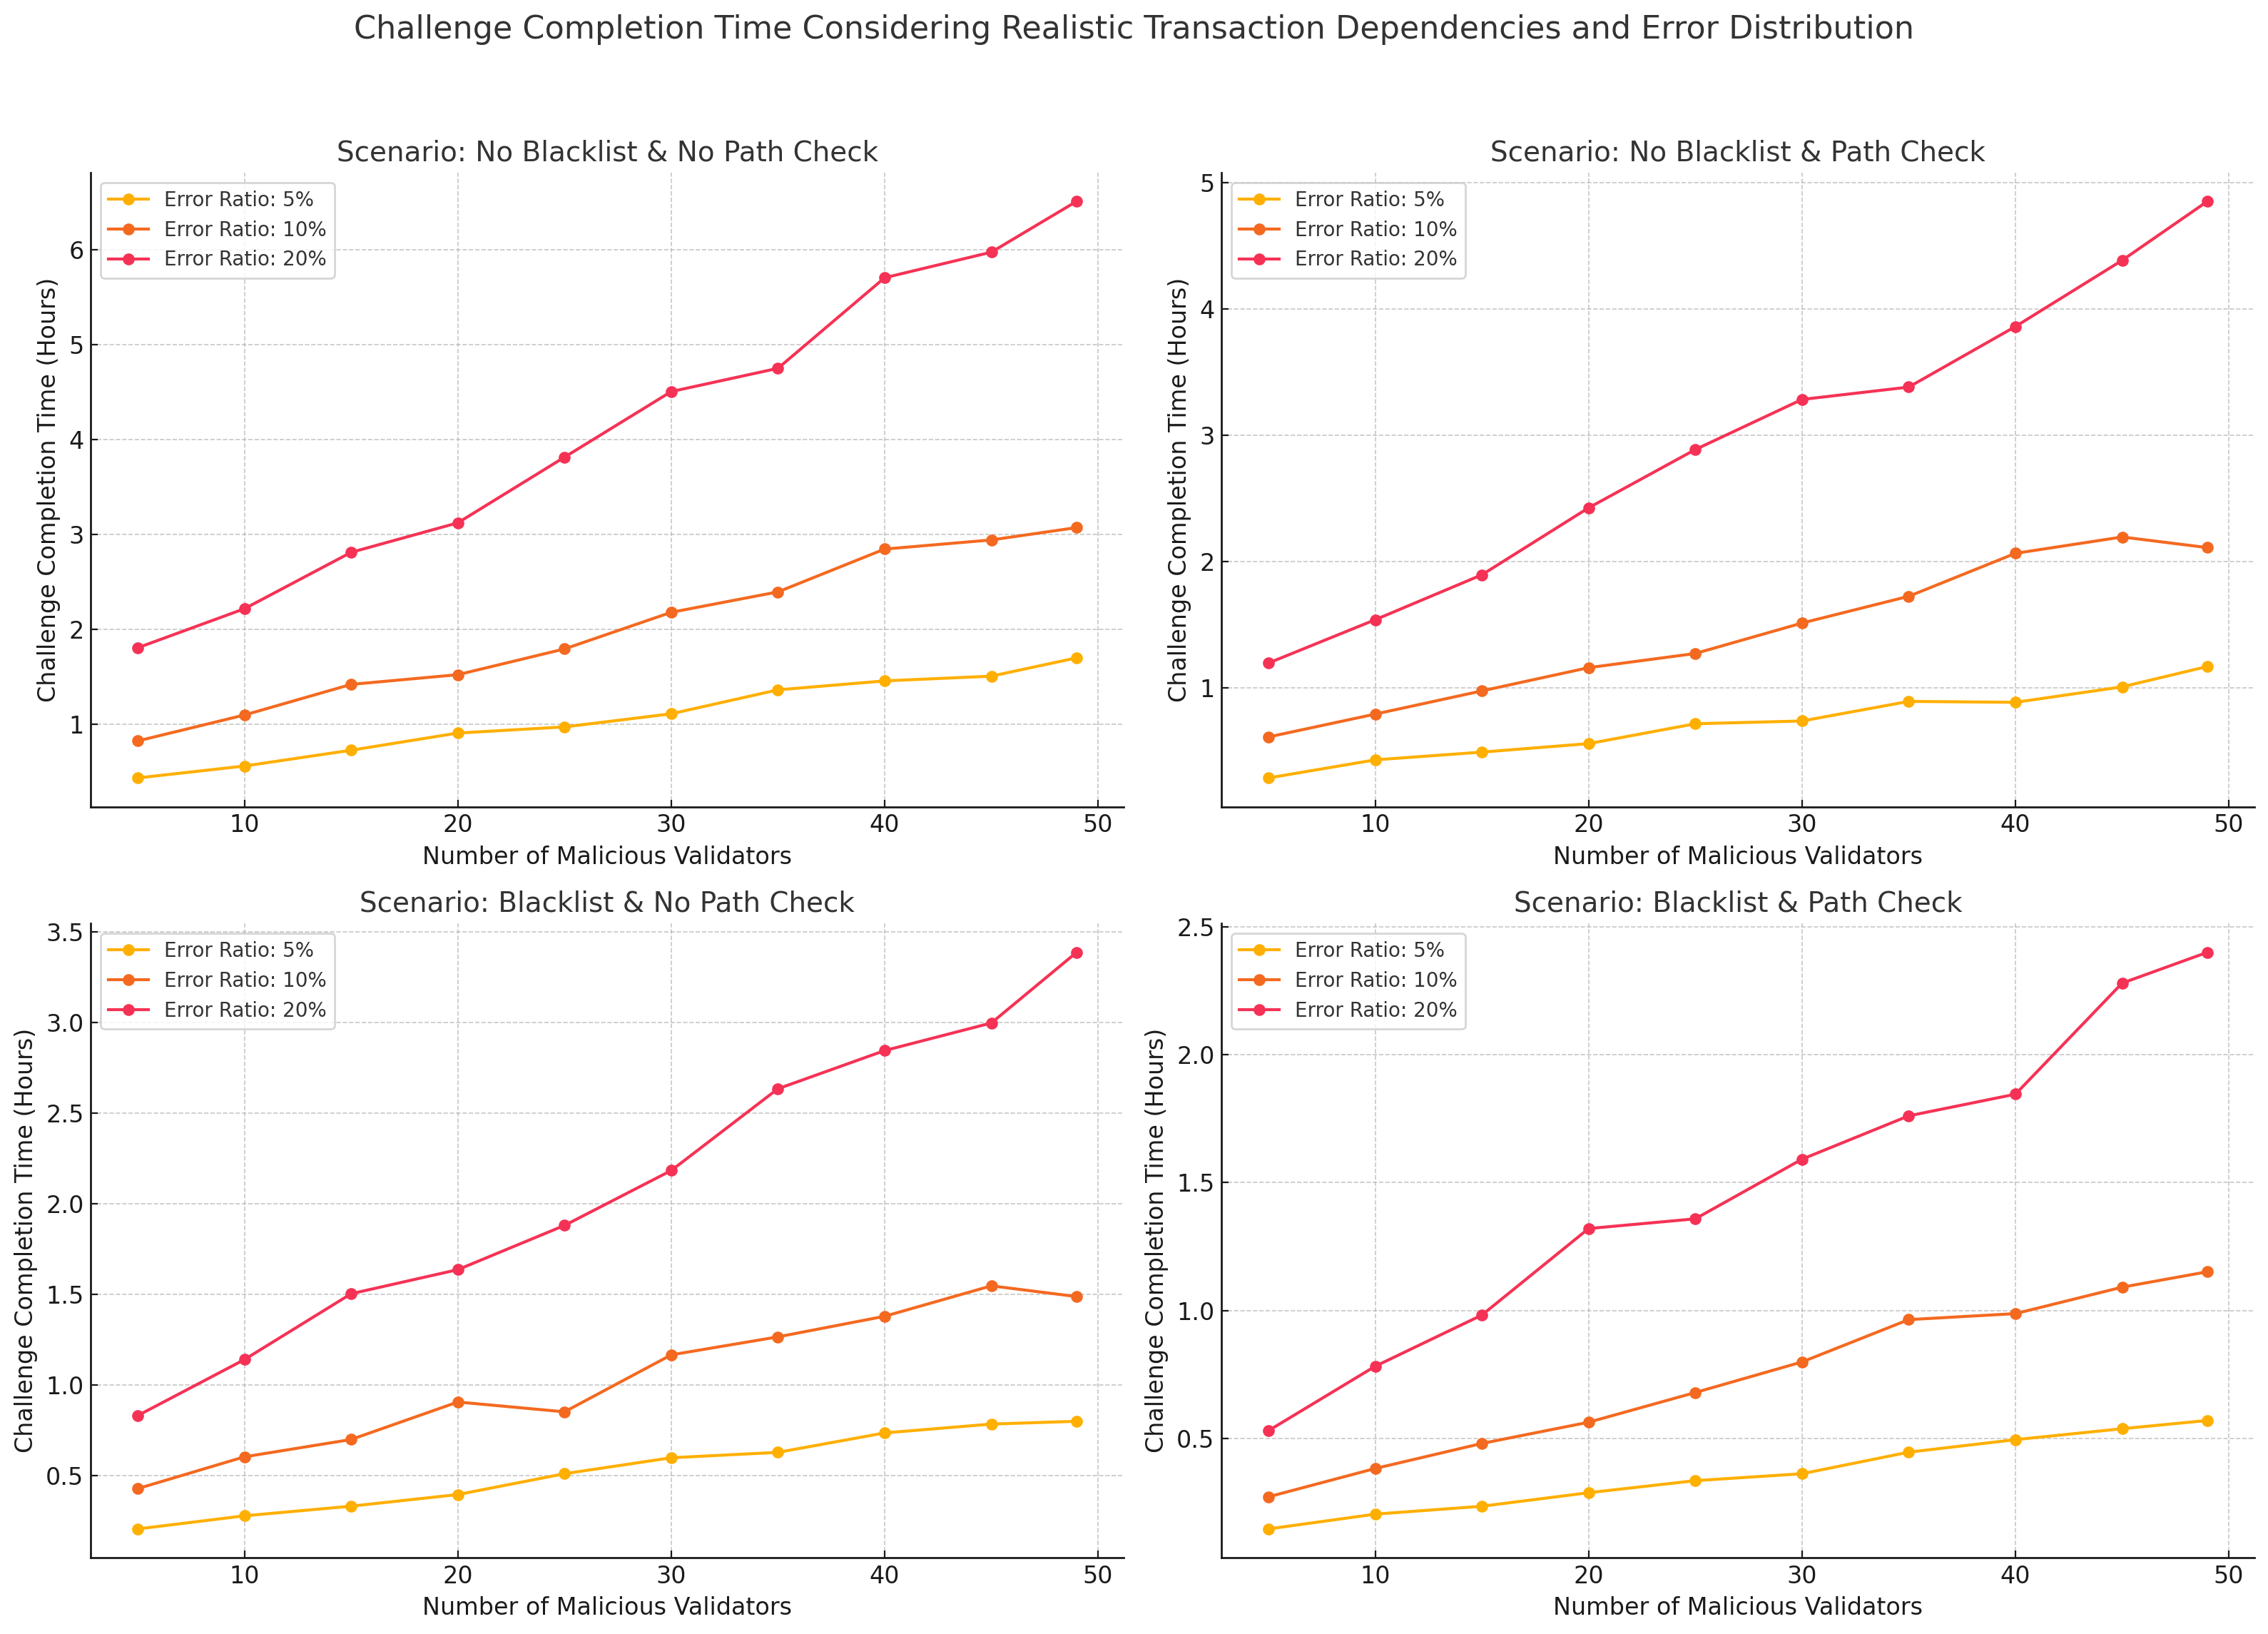
\includegraphics[width=1.0\linewidth]{window.png}
\caption{Challenge Window Duration under Various Optimization Mechanisms}
\label{fig:time}
\end{figure}

Figure~\ref{fig:time} shows that the unoptimized challenge window ranges from 72.0 s to 210.0 s under the tested error ratios, while the combined optimization reduces it to 50.7 s, 67.0 s, and 94.3 s, respectively. The maximum reduction reaches 55.1\% at a 20\% error ratio, indicating that path pruning and verifier blacklisting keep dispute handling within a short, testable time window.


\section{Conclusion and Future Work}

This paper presents \textbf{AnoST}, an anonymous optimistic verification framework for rollup-based blockchains. By integrating anonymous staking-based verifier election with state-centric verification primitives—namely, the State Transition Commitment (STC) and State Transition Tree (STT)—AnoST addresses verifier identity exposure, the Verifier's Dilemma, and coarse-grained rollback limitations. Experimental results confirm its strong anonymity guarantees, enhanced verifier participation, and scalable, fine-grained rollback support.

Future extensions include enhancing AnoST against adaptive verifier collusion, designing robust incentive-compatible reward models, and addressing integration challenges in real-world rollup systems (e.g., Arbitrum, Optimism). These efforts aim to advance AnoST toward scalable and privacy-preserving Layer 2 deployments.


\begin{credits}
\subsubsection{\ackname} This paper is supported by the National Key R\&D Program of China through project 2022YFB2702900, the Natural Science Foundation of China through projects U21A20467, U24B20144 and 62272464.
\end{credits}


\bibliographystyle{splncs04}
\bibliography{mybibliography}


\end{CJK*}
\end{document}
